\documentclass[aspectratio=169]{beamer}

\usetheme{Boadilla}
\usecolortheme{seahorse}
\setbeamertemplate{navigation symbols}{}
\setbeamertemplate{footline}[frame number]

\usepackage[T1]{fontenc}
\usepackage[utf8]{inputenc}
\usepackage{booktabs}
\usepackage{graphicx}
\usepackage{amsmath}
\usepackage{array}
\pdfstringdefDisableCommands{%
  \def\translate#1{#1}%
}

\definecolor{DeepTeal}{RGB}{38,105,110}
\definecolor{SoftGray}{RGB}{245,247,248}
\definecolor{DarkText}{RGB}{34,41,47}
\setbeamercolor{title}{fg=DeepTeal}
\setbeamercolor{frametitle}{fg=DeepTeal}
\setbeamercolor{structure}{fg=DeepTeal}
\setbeamercolor{normal text}{fg=DarkText}
\setbeamercolor{block title}{bg=DeepTeal,fg=white}
\setbeamercolor{block body}{bg=SoftGray,fg=DarkText}

\newcommand{\metric}[1]{\textbf{\color{DeepTeal}#1}}
\newcommand{\smalltab}{\scriptsize}

\title[Adaptive Evidence for Grounded VideoQA]{Adaptive Evidence Acquisition for Grounded Video Question Answering}
\author{Aniket Salunke \and Ketan More \and Nazish Baliyan \and Ritesh Thawkar}
\institute{Mohamed Bin Zayed University of Artificial Intelligence}
\date{Final Presentation}

\begin{document}

\begin{frame}
  \titlepage
\end{frame}

\begin{frame}{Motivation}
  \begin{columns}[T,onlytextwidth]
    \begin{column}{0.56\textwidth}
      \begin{block}{Core issue}
        VideoQA systems often answer from a fixed amount of visual context, even when the answer depends on a short event.
      \end{block}
      \vspace{0.5em}
      This creates two problems:
      \begin{itemize}
        \item computation is spent on irrelevant frames;
        \item a correct answer may not be grounded in the supporting moment.
      \end{itemize}
    \end{column}
    \begin{column}{0.39\textwidth}
      \begin{block}{Research question}
        How much visual evidence is enough to answer a video question while staying temporally grounded?
      \end{block}
    \end{column}
  \end{columns}
\end{frame}

\begin{frame}{Related Work and Gap}
  \begin{columns}[T,onlytextwidth]
    \begin{column}{0.48\textwidth}
      \textbf{What prior work gives us}
      \begin{itemize}
        \item VideoQA benchmarks: MovieQA, TGIF-QA, TVQA, NExT-QA.
        \item Vision-language pretraining: CLIP, VideoCLIP, CLIP4Clip.
        \item Grounded VideoQA: NExT-GQA asks whether answers are supported by visual evidence.
      \end{itemize}
    \end{column}
    \begin{column}{0.48\textwidth}
      \textbf{Gap we study}
      \begin{itemize}
        \item Most systems use fixed context or fixed top-$K$ retrieval.
        \item Retrieval quality, answer accuracy, and grounding are often evaluated separately.
        \item We evaluate them together as an evidence-acquisition tradeoff.
      \end{itemize}
    \end{column}
  \end{columns}
\end{frame}

\begin{frame}{Problem Formulation}
  A grounded VideoQA example is:
  \[
    x = (v, q, \mathcal{A}, y, \mathcal{T})
  \]
  \vspace{-0.5em}
  \begin{itemize}
    \item $v$: video, $q$: question, $\mathcal{A}$: answer options.
    \item $y$: correct answer, $\mathcal{T}$: temporal grounding span.
    \item Candidate evidence pool: $\mathcal{E}(x)=\{e_1,\ldots,e_N\}$.
  \end{itemize}

  \vspace{0.5em}
  A policy selects evidence $S \subseteq \mathcal{E}(x)$ with cost:
  \[
    C(S)=\sum_{e_i \in S} c_i
  \]

  \begin{block}{Goal}
    Maximize answer accuracy and temporal grounding while minimizing acquired evidence cost.
  \end{block}
\end{frame}

\begin{frame}{Method}
  \centering
  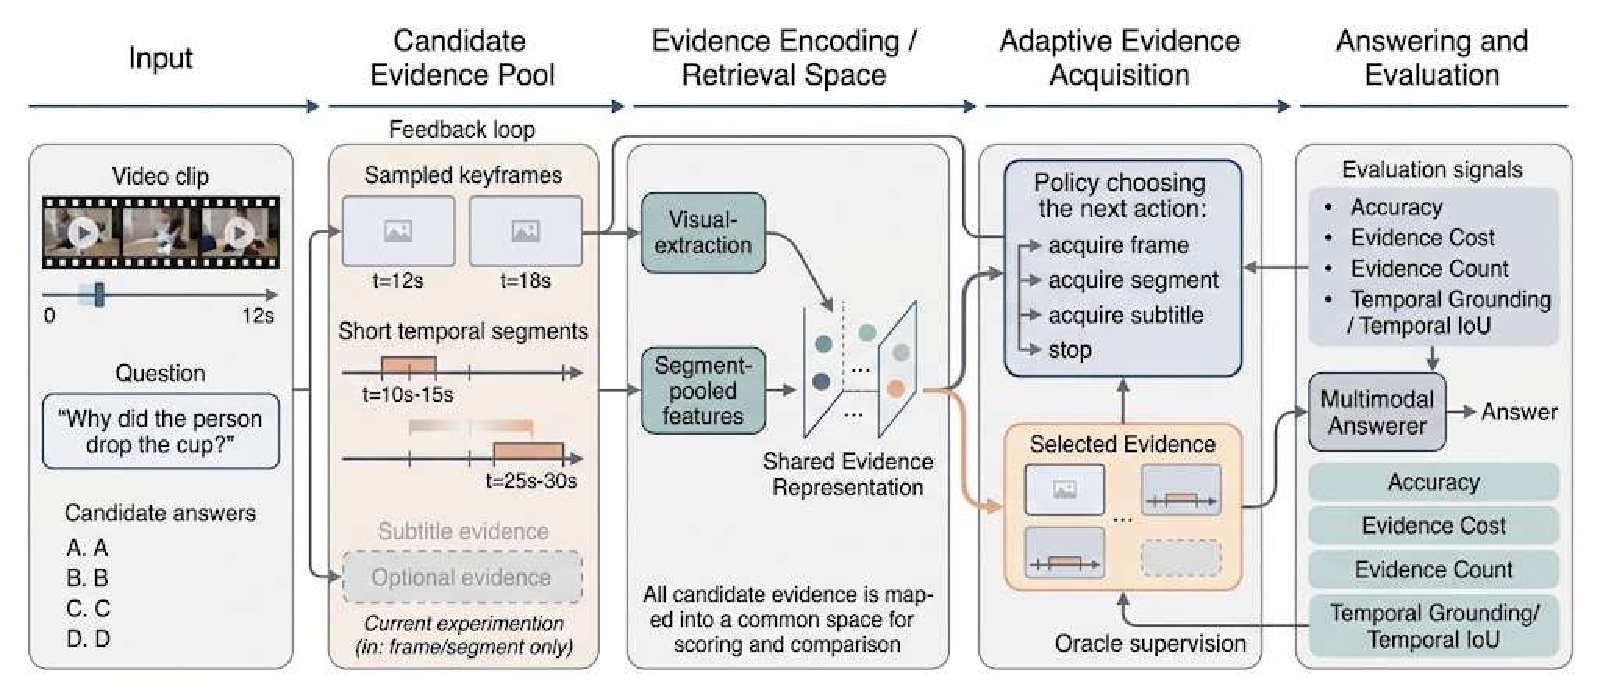
\includegraphics[width=0.84\linewidth]{../report/figure_1.pdf}

  \vspace{0.1em}
  \small
  \begin{itemize}
    \item Build frame and short segment evidence candidates from NExT-GQA videos.
    \item Compare one-segment, learned two-item, and fixed-budget evidence policies.
    \item Re-answer the same evidence using a frozen CLIP-style answerer and Qwen2.5-VL.
  \end{itemize}
\end{frame}

\begin{frame}{Evaluation Protocol}
  \begin{columns}[T,onlytextwidth]
    \begin{column}{0.50\textwidth}
      \textbf{Dataset and controls}
      \begin{itemize}
        \item NExT-GQA validation: 3,358 examples.
        \item NExT-GQA test: 5,553 examples.
        \item Evidence policies:
          \begin{itemize}
            \item one segment;
            \item learned two-item policy;
            \item fixed 3 frames + 3 segments.
          \end{itemize}
      \end{itemize}
    \end{column}
    \begin{column}{0.46\textwidth}
      \textbf{Metrics}
      \begin{itemize}
        \item Acc@QA: answer accuracy.
        \item Cost and evidence count.
        \item mIoP, IoP@0.5, mIoU, IoU@0.5.
        \item Acc@GQA: correct answer and IoP $\geq 0.5$.
      \end{itemize}
      \vspace{0.3em}
      \footnotesize Acc@GQA is computed over the selected evidence set.
    \end{column}
  \end{columns}
\end{frame}

\begin{frame}{Result 1: Frozen Answerer Is the Bottleneck}
  \begin{table}
    \centering
    \smalltab
    \begin{tabular}{lrrrr}
      \toprule
      Method & Acc@QA & Cost & IoP@0.5 & Acc@GQA \\
      \midrule
      One segment & 0.378 & 1.500 & 0.311 & 0.124 \\
      Learned two-item policy & 0.381 & 2.795 & 0.410 & 0.164 \\
      Fixed 3 frames + 3 segments & 0.388 & 7.500 & 0.615 & 0.245 \\
      Fixed 6 frames + 6 segments & 0.394 & 14.908 & 0.787 & 0.316 \\
      \bottomrule
    \end{tabular}
  \end{table}

  \begin{block}{Takeaway}
    The learned policy improves grounding, but answer accuracy remains near 0.38 because the frozen answerer is too weak.
  \end{block}
\end{frame}

\begin{frame}{Result 2: Stronger Answerer Reveals the Tradeoff}
  \begin{table}
    \centering
    \smalltab
    \begin{tabular}{lrrrr}
      \toprule
      Method & Acc@QA & Cost & IoP@0.5 & Acc@GQA \\
      \midrule
      Qwen one segment & 0.674 & 1.500 & 0.315 & 0.225 \\
      Qwen learned two-item policy & 0.695 & 2.785 & 0.415 & 0.302 \\
      Qwen fixed 3 frames + 3 segments & 0.724 & 7.500 & 0.615 & 0.457 \\
      \bottomrule
    \end{tabular}
  \end{table}

  \begin{itemize}
    \item Learned two-item evidence keeps \metric{96\%} of fixed 3+3 answer accuracy.
    \item It uses only \metric{37\%} of the evidence cost.
    \item It keeps only about \metric{66\%} of fixed 3+3 grounded answer accuracy.
  \end{itemize}
\end{frame}

\begin{frame}{Full Test-Set Summary}
  \begin{table}
    \centering
    \scriptsize
    \setlength{\tabcolsep}{3pt}
    \begin{tabular}{lrrrr}
      \toprule
      Method & Acc@QA & Cost & IoP@0.5 & Acc@GQA \\
      \midrule
      Qwen one segment & 0.668 & 1.500 & 0.311 & 0.221 \\
      Qwen learned two-item policy & 0.696 & 2.795 & 0.410 & 0.297 \\
      Qwen fixed 3 frames + 3 segments reference & 0.724 & 7.500 & 0.615 & 0.454 \\
      \bottomrule
    \end{tabular}
  \end{table}

  \begin{block}{Takeaway}
    The test-set summary preserves the central tradeoff: learned evidence is the better budgeted method, while fixed 3+3 remains the high-coverage grounding reference.
  \end{block}
\end{frame}

\begin{frame}{Accuracy-Cost-Grounding Tradeoff}
  \centering
  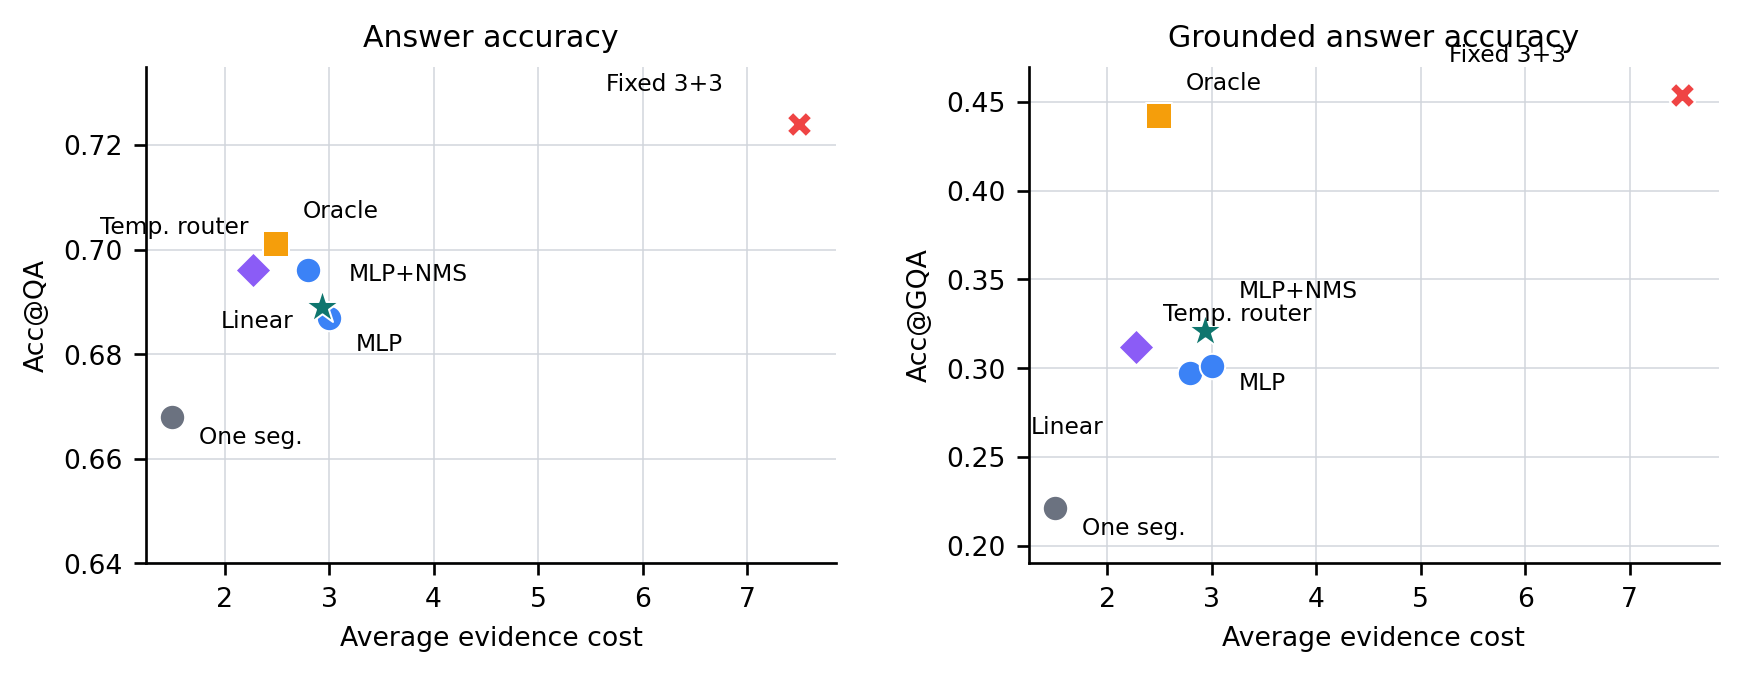
\includegraphics[width=0.78\linewidth]{../report/qwen_current_tradeoff_presentation.png}

  \vspace{-0.1em}
  \begin{block}{Interpretation}
    Compact evidence is efficient for answering, but faithful grounding still benefits from more temporal coverage.
  \end{block}
\end{frame}

\begin{frame}{Qualitative Lessons}
  \begin{table}
    \centering
    \scriptsize
    \setlength{\tabcolsep}{3pt}
    \begin{tabular}{p{0.23\linewidth}p{0.42\linewidth}p{0.25\linewidth}}
      \toprule
      Case & Question & Outcome \\
      \midrule
      Correct and grounded &
      Why is the boy in yellow reaching out to things on the green mat? &
      Predicted C, gold C; temporal IoU 0.675 \\
      Correct, weakly grounded &
      Why did the boy pick up one present and move to the sofa? &
      Predicted C, gold C; temporal IoU 0.047 \\
      Grounded but wrong &
      Why did the man in white hold tightly to the boy in white? &
      Predicted E, gold D; temporal IoU 0.541 \\
      \bottomrule
    \end{tabular}
  \end{table}

  \begin{block}{Lesson}
    Answer correctness and temporal grounding are related but not interchangeable.
  \end{block}
\end{frame}

\begin{frame}{Conclusion}
  \begin{block}{Main conclusion}
    Grounded VideoQA should be evaluated as evidence selection plus answering, not only answer classification.
  \end{block}

  \begin{itemize}
    \item A weak answerer hides meaningful evidence-policy differences.
    \item Qwen2.5-VL makes compact evidence useful for answering.
    \item Fixed larger evidence still wins when grounding is the priority.
    \item The final result is an accuracy-cost-grounding tradeoff, not a single winner.
  \end{itemize}

  \vspace{0.5em}
  \footnotesize The full test-set summary states the final accuracy-cost-grounding tradeoff used for today's presentation.
\end{frame}

\appendix

\begin{frame}{Backup: Official Metric Caveat}
  \begin{itemize}
    \item NExT-GQA official grounding code expects one predicted temporal span per question.
    \item Our method selects a set of evidence items.
    \item The report uses a transparent evidence-set metric: best selected evidence item with IoP $\geq 0.5$.
    \item A single-span version requires an aggregation rule such as first selected span, highest-score span, or union span.
  \end{itemize}

  \begin{block}{How to discuss this in Q\&A}
    We do not claim official single-span leaderboard comparability; we use the metric to study evidence-set support under controlled policies.
  \end{block}
\end{frame}

\begin{frame}{Backup: Result Provenance}
  \begin{itemize}
    \item Test split size: 5,553 examples.
    \item The one-segment row comes from the generated Qwen test predictions.
    \item The learned row is a completed full-test result.
    \item The fixed 3+3 row is the high-cost coverage reference.
  \end{itemize}

  \begin{block}{How to discuss this in Q\&A}
    The research conclusion depends on the ordering across operating points and the large cost gap, not on small changes in the final decimal places.
  \end{block}
\end{frame}

\end{document}
